% Copyright (C) 2014 by Thomas Auzinger <thomas.auzinger@cg.tuwien.ac.at>

\documentclass[draft,final]{vutinfth} % Remove option 'final' to obtain debug information.

% Extended LaTeX functionality is enables by including packages with \usepackage{...}.
\usepackage{fixltx2e}  % Provides fixes for several errors in LaTeX2e.
\usepackage{amsmath}   % Extended typesetting of mathematical expression.
\usepackage{amssymb}   % Provides a multitude of mathematical symbols.
\usepackage{mathtools} % Further extensions of mathematical typesetting.
\usepackage{microtype} % Small-scale typographic enhancements.
\usepackage{enumitem}  % User control over the layout of lists (itemize, enumerate, description).
\usepackage{multirow}  % Allows table elements to span several rows.
\usepackage{booktabs}  % Improves the typesettings of tables.
\usepackage[ruled,linesnumbered,algochapter]{algorithm2e} % Enables the writing of pseudo code.
\usepackage{nag}       % Issues warnings when best practices in writing LaTeX documents are violated.
\usepackage{hyperref}  % Enables cross linking in the electronic document version. This package has to be included second to last.
\usepackage[acronym,toc]{glossaries} % Enables the generation of glossaries and lists fo acronyms. This package has to be included last.
\usepackage{tikz}
\usepackage{placeins}
\usepackage{amsmath}
\usepackage[nounderscore]{syntax}
\usepackage[style=ieee, backend=bibtex]{biblatex}
\usepackage{csquotes}
\usepackage{hyperref}

\AtBeginDocument{\renewcommand{\bibname}{References}} % rename bibliography to references
\bibliography{bakk}

\newcommand{\hl}{\par\vspace{6pt}} %used within the same context, as new paragraph
\newcommand{\cl}{\par\vspace{12pt}} %used between paragraphs with the same topic, but not textually flowing into each other
\setlength{\parindent}{0pt} %should remove all intendations

\setsecnumdepth{subsection} % enumerate subsections

% Use an optional index
\makeindex
% Use an optional glossary
%\makeglossaries
%\glstocfalse % remove the glossaries from the table of contents

% Set persons with 4 arguments:
%  {title before name}{name}{title after name}{gender}
%  where both titles are optional (i.e. can be given as empty brackets {})
\setauthor{}{Patrick Bellositz}{}{male}
\setadvisor{Ao.Prof.Dipl.-Ing.Dr.techn.}{Christian Georg Ferm{\"u}ller}{}{male}

% Required data
\setaddress{Eichkogelstra{\ss}e 10/10/9, 2353 Guntramsdorf}
\setregnumber{1027108}
\setdate{01}{06}{2015}
\settitle{Argumentation Frameworks}{Argumentation Frameworks} % sets English and German version of the title (both can be English or German)

\setthesis{bachelor}

% For bachelor and master
\setcurriculum{Software \& Information Engineering}{Software \& Information Engineering} % sets the English and German name of the curriculum

\begin{document}

\frontmatter % switches to roman numbering
% The structure of the thesis has to conform to
%  http://www.informatik.tuwien.ac.at/dekanat

%\addtitlepage{naustrian}
\addtitlepage{english} % English title page
\addstatementpage

\begin{acknowledgements*}
I want to thank my family for supporting me and Dr. Ferm{\"u}ller for guiding me in the process of creating this thesis.
\end{acknowledgements*}

\begin{abstract*}
This bachelor thesis explains argumentation frameworks and provides their most important semantics. It further analyzes the relations between different types of extension semantics.\hl
The main part of this thesis is the the developement of a JAVA application which is capable of creating custom argumentation frameworks, their representation as graphs and the computation of extensions. The application is created in a way such that students can study argumentation frameworks in an easily digestable way including step-by-step explanations of how to compute extensions accompanied by coloured highlighting of important aspects of the frameworks' graphs.
\end{abstract*}

% Select the language of the thesis, e.g., english or naustrian.
\selectlanguage{english}

% Add a table of contents (toc)
\tableofcontents* % starred version, i.e., \tableofcontents*, removes the self-entry

% Switch to arabic numbering and start the enumeration of chapters in the table of content.
\mainmatter

\chapter{Introduction}
Most humans argue daily. An argument is made, which is followed by a counter-argument and so on until there is a resolution. This way decisions can be made that satisfy the needs of the arguing parties, be it in a large group of people or a single person weighing all the information they have, the decision depending on the arguments that ``win''.\hl
In 1995 Dung introduced \emph{argumentation frameworks} as a basic theory to implement human argumentation mechanisms on computers in \cite{Dung}.\cl
First we will define argumentation frameworks and analyse semantics for them representing both credulous and sceptical approaches to reasoning. An example is provided to illustrate the diffences in computing the sets (called extensions) these semantics yield.\hl
Next we examine how the different extension types are related to each other. We also will look at additional semantics and compare them to Dung's original ones they build upon using additional examples.\hl
In the last chapter we take a look at a computer program, specifically written along with this bachelor thesis, that allows the user to define argumentation frameworks (or, alternatively, choose from a set of examples) and that explains how the extensions of these frameworks are computed.\cl
The goal of this thesis is to enable students to more easily acquire knowledge about argumentation frameworks by giving them the necessary information and providing them with a tool to aid them in their understanding of this topic.

\chapter{Definitions}

To work with argumentation frameworks, first we must define their properties. In this section we will introduce the basic semantics for argumentation frameworks. If not otherwise mentioned the following definitions were proposed by Dung in \cite{Dung}.\cl

\section{Argumentation Frameworks}

First we define argumentation frameworks as pairs of arguments and attacks relations.\hl

\textbf{Definition 1.} An \emph{argumentation framework} $F$ is a pair $(A,R)$, where $A$ is a set of arguments and $R$ is an attack relation.\cl

The aforementioned attacks are defined as follows.\hl

\textbf{Definition 2.} An \emph{attack relation} $R\subseteq A\times A$ is a set of pairs $(a,b)$, where $a,b\in A$ means $a$ \emph{attacks} $b$.\cl

\textbf{Remark 1.} Let $S$ be a set of arguments. If $a\in S$ and there is an attack $(a,b)\in R$ we say $S$ \emph{attacks} $b$.\cl

\textbf{Example 1.} Imagine we have three arguments $a_1$, $a_2$, and $b$.\hl
			\begin{tabular}{p{0.5cm}p{0.5cm}l}
			& $a_1$ & = ''Blue is the most beautiful of all colours.''\\
			& $b$ & = ''No, black is much more beautiful!''\\
			& $a_2$ & = ''That's wrong, black isn't even a colour.''
			\end{tabular}\hl
We can see that argument $b$ attacks argument $a_1$ and vice versa. Additionally argument $a_2$ attacks argument $b$.\hl
This results in the framework $F=(A,R)$, where $A=\{a_1,a_2,b\}$ and $R=\{(b,a_1),(a_1,b),(a_2,b)\}$.\cl

It is also possible to represent every framework as a graph $(V,E)$, where $V=A$ and $E=R$. The graph representing the framework in our example looks like this:

\FloatBarrier
	\begin{figure}[!ht]
		\centering
		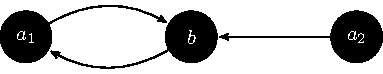
\includegraphics[width=\linewidth]{graphs/ex1_v2.pdf}
		\caption{An argumentation framework about colours.}
	\end{figure}
\FloatBarrier

\textbf{Remark 2.} From now on, when mentioning $A$ or $R$, we refer to the sets of an arbitrary, fixed argumentation framework $F=(A,R)$, unless otherwise stated.\cl

The semantics of argumentation frameworks is captured by singling out certain so-called extensions intended to collect maximal subsets of arguments that are jointly maintainable according to various criteria with respect to the other arguments present in the argumentation framework.\cl

\section{Conflict-free sets}

As a basis for extensions we introduce \emph{conflict-free sets}. Since no extension should contain arguments that are in conflict with each other, there should be no attack consisting of two arguments of the same set.\cl

\textbf{Definition 3.} Given an argumentation framework $F=(A,R)$, let $S\subseteq A$ be a set of arguments. It is \emph{conflict-free}, if $\nexists (a,b)\in R$, where $a,b\in S$.\\
The set of all conflict-free sets of $F$ is denoted $cf(F)$.\cl

\textbf{Example 2.} (Continuation of Example 1.) As no argument attacks itself, $\{a_1\}$, $\{a_2\}$ and $\{b\}$ each are conflict-free. $\{a_1,a_2\}$ is also a conflict-free set, since there exists no attack consisting of both $a_1$ and $a_2$. The empty set is always conflict-free.\hl
Since there is an attack between $b$ and each of the other arguments, there are no other conflict-free sets.\hl
It follows that $cf(F)=\{\emptyset,\{a_1\},\{a_2\},\{b\},\{a_1,a_2\}\}$.\cl

\section{Admissible extensions}

To be able to find a set of arguments that can defend itself, it does not suffice that a set is not in conflict with itself. Additionally each of its arguments should also be defended from outside attackers as is the case with admissible semantics.\hl

\textbf{Definition 4.} An argument $a$ is \emph{defended} by a set $S$, iff for every attack $(b,a)\in R$ there is an attack $(c,b)$, where $c\in S$.\cl

\textbf{Definition 5.} Let $S$ be a conflict-free set. It is called an \emph{admissible extension} if it defends each $a\in S$.\\
The set of all admissible extensions of an argumentation framework $F$ is denoted $adm(F)$.\cl

\textbf{Example 3.} (Continuation of Example 2.) Of the conflict-free sets only \(\emptyset\) and $\{a_2\}$ don't get attacked. Therefore they are admissible extensions. $\{a_1\}$ defends itself from its only attacker $b$ via the attack $(a_1,b)$, making it an admissible extension. $\{a_1,a_2\}$ gets attacked via the attack $(b,a_1)$, but $a_1$ gets defended through $(a_1,b)$ and $(a_2,b)$, also making it an admissible extension.\\
$\{b\}$ is not admissible since it doesn't defend its argument against the attacks by $a_1$ and $a_2$.\hl
It follows that $adm(F)=\{\emptyset,\{a_1\},\{a_2\},\{a_1,a_2\}\}$.\cl

\section{Preferred extensions}

Most given argumentation frameworks produce big numbers of admissible extension. Preferred semantics reduce the number of extensions, only taking the biggest ones. The resulting preferred extensions represent a credulous approach of reasoning, since they contain all arguments that are contained in admissible extensions.\hl
They were defined in \cite{Egly} as follows:\cl

\textbf{Definition 6.} Let $S$ be an admissible extension. It is called a \emph{preferred extension} if for each $S'\subseteq A$, that is an admissible extension, $S\not\subset S'$.\\
The set of all preferred extensions of an argumentation framework $F$ is denoted $prf(F)$.\cl

\textbf{Example 4.} (Continuation of Example 3.) Since $\emptyset\subset\{a_2\}$, \(\emptyset\) is not a preferred extension. Since $\{a_1\}\subset\{a_1,a_2\}$ and $\{a_2\}\subset\{a_1,a_2\}$, $\{a_1\}$ and $\{a_2\}$ are not a preferred extensions. Since all other admissible extensions are proper subsets of $\{a_1,a_2\}$, it is a preferred extension.\hl
It follows that $prf(F)=\{\{a_1,a_2\}\}$.\hl
As we can see, all arguments contained in admissible extensions still are contained in a preferred extension.\cl

\section{Stable extensions}

Additionally we can define a stricter version of the admissible extension, that not only requires arguments to be defended, but also attacks all arguments not contained within it.\cl

\textbf{Definition 7.} Let $S$ be a conflict-free set. It is called a \emph{stable extension} if for each $a\not\in S$ there exists an attack $(b,a)\in R$ where $b\in S$.\\
The set of all stable extensions of an argumentation framework $F$ is denoted $st(F)$.\cl

\textbf{Example 5.} (Continuation of Example 2) The conflict-free set $\emptyset$ doesn't attack any of the other arguments, $\{a_1\}$ and $\{a_2\}$ only attack $b$, not attacking $a_2$ or $a_1$ respectively. $\{b\}$ doesn't attack $a_2$. Since they don't attack all arguments they don't contain, these sets are not stable extensions.\\
$\{a_1,a_2\}$ attacks the only other argument (i.e. $b$, via attack $(a_2,b)$) and therefore is a stable extension.\hl
It follows that $st(F)=\{\{a_1,a_2\}\}$.\cl

\section{Complete extensions}

Credulous reasoning contrasts sceptical reasoning. An extension matching sceptical reasoning within the context of argumentation frameworks is the complete extension.\cl

\textbf{Definition 8.} Let $S$ be an admissible extension. It is called a \emph{complete extension} if for each $a\not\in S$, $S$ does not defend $a$.\\
The set of all complete extensions of an argumentation framework $F$ is denoted $co(F)$.\cl

\textbf{Example 6.} (Continuation of Example 3.) The admissible extension $\emptyset$ is not a complete extension because it defends $a_2$ which it doesn't contain. The same is true for $\{a_1\}$. $\{a_2\}$ defends $a_1$ and is therefore also not a complete extension.\\
$\{a_1,a_2\}$ attacks $b$ and as there are no other arguments which could be defended it is a complete extension.\hl
It follows that $co(F)=\{\{a_1,a_2\}\}$.\cl

\section{Grounded extension}

As before, we can again reduce the number of extensions. In this case we search for the common denominator, meaning exactly those arguments all complete extensions can ``agree'' on. This set is called the grounded extension as defined in \cite{Egly}.\cl

\textbf{Definition 9.} The (unique) \emph{grounded extension} is defined by $\bigcap\limits_{i=1}^n{S_i}$, where $\{S_1,...,S_n\}$ is the set of all complete extensions.\\
The grounded extension of an argumentation framework $F$ is denoted $gr(F)$\cl

\textbf{Example 7.} (Continuation of Example 6.) Since there is only one complete extension $\{a_1,a_2\}$, it also is the grounded extension $gr(F)$.\cl

\chapter{Relations and additional semantics}

As we have seen in the previous chapter, there often are sets meeting the criteria for more than one extension type. In this chapter we look at the relations between extension types, explore their features and provide additional extension semantics. In advance the relations between extension types, including additional extension types, are shown in Figure 3.1 which was adapted from \cite{Gorogiannis}.\cl

\FloatBarrier
	\begin{figure}[!h]
		\centering
		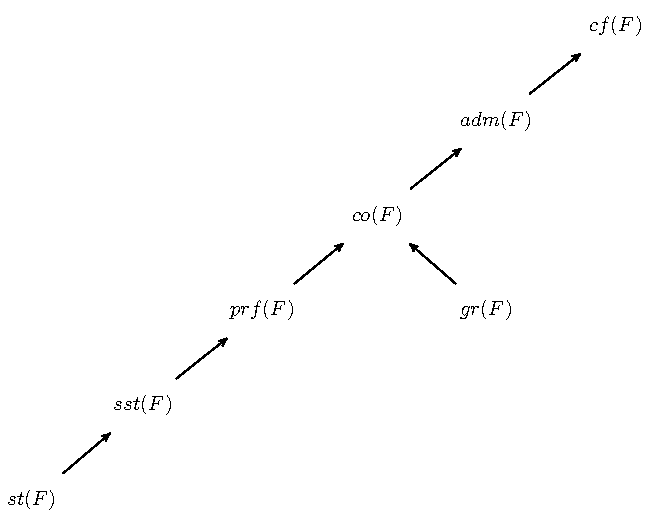
\includegraphics[scale=1]{graphs/diagram_2.pdf}
		\caption[Relations between sets of an argumentation framework]{Relations between sets of an argumentation framework. An arrow from X to Y means that, if a set is X it also is Y}
	\end{figure}
\FloatBarrier

\section{Relations between extension types}
In this section we will examine relations between different types of extensions.\hl

As per the definitions of the extensions there are the following relations:
\begin{align}
	adm(F)\subseteq cf(F)  \\ \label{eq1}
	st(F)\subseteq cf(F) \\
	prf(F)\subseteq adm(F)\\
	co(F)\subseteq adm(F)
\end{align}\cl

Additional to relations already given in their definitions, there are further relations to be mentioned.\hl
The following Lemma is provided in \cite{Dung} and regards the relation between stable and preferred extensions.\cl

\textbf{Lemma 1.}
Each stable extension is a preferred extension, but not every preferred extension is a stable extension.
\begin{align}
	st(F)\subseteq prf(F)\\
	prf(F)\not\subseteq st(F)
\end{align}
Therefore each stable extension also is an admissible extension.\cl

\textbf{Example 8.} Let $F$ be an argumentation framework $(A,R)$ such that $A=\{a,b,c\}$ and $R=\{(b,a),(b,c),(a,a),(c,b)\}$.\hl

\FloatBarrier
	\begin{figure}[!h]
		\centering

		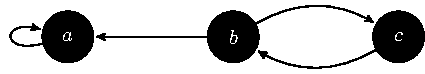
\includegraphics[width=\linewidth]{graphs/ex2_v2.pdf}
		\caption{An argumentation framework $F$, where $st(F)\subsetneq prf(F)$}
	\end{figure}
\FloatBarrier

It can be computed that $cf(F)=adm(F)=\{\emptyset,\{b\},\{c\}\}$. So we only have to consider three extensions for further computations.\hl
As can be seen, $\{b\}$ is the only conflict-free set that attacks all other arguments. Therefore $st(F)=\{\{b\}\}$ and it becomes obvious that $st(F)\subsetneq prf(F)$.\cl

Further we look at the relation between preferred, complete and grounded extensions. Dung provides the following Lemma in \cite{Dung}.\hl

\textbf{Lemma 2.}
Each preferred extension is a complete extension, but not vice versa.
\begin{align}
	\label{eq7} prf(F)\subseteq co(F) \\ 
	\label{eq8} co(F)\not\subseteq prf(F) 
\end{align}\hl

\textbf{Example 9.} Let $F$ be an argumentation framework $(A,R)$ such that $A=\{a,b,c,d\}$ and $R=\{(a,b),(b,a),(c,b),(c,d),(d,c)\}$.\hl

\FloatBarrier
	\begin{figure}[!h]
		\centering
		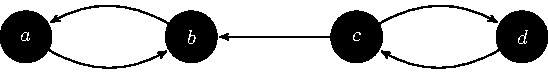
\includegraphics[width=\linewidth]{graphs/ex3.pdf}
		\caption{An argumentation framework $F$, where $prf(F)\subset co(F)$}
	\end{figure}
\FloatBarrier

To compute complete extensions as well as preferred extensions we use the set of admissible extensions $adm(F)=\{\emptyset,\{a\},\{c\},\{d\},\{a,c\},\{a,d\},\{b,d\}\}$.\hl
All admissible extensions except $\{c\}$ contain all the arguments they defend. Hence they are complete. $\{c\}$ defends $a$, which it doesn't contain and therefore is not complete. It follows that $co(F)=\{\emptyset,\{a\},\{d\},\{a,c\},\{a,d\},\{b,d\}\}$\hl
Of the admissible extensions $\emptyset,\{a\}$ and $\{d\}$ are subsets of $\{a,d\}$, while $\{c\}$ is a subset of $\{a,c\}$. Those are not preferred extensions. We get $prf(F)=\{\{a,c\},\{a,d\},\{b,d\}\}$, since these sets are not subsets of each other.\hl
As we can see (\ref{eq7}) and (\ref{eq8}) are both satisfied.\cl

Regarding the relation between grounded and complete extensions,\cite{Dung} contains the following information:\hl

\textbf{Lemma 3.} The grounded extension is the least (w.r.t. set inclusion) complete extension.
\begin{align}
	gr(F)\in co(F)
\end{align}\cl

\section{Additional semantics}
In this section we will look at a few additional extension semantics and how they relate to the ones mentioned above.

\subsection{Semi-stable extensions}
The only one of Dung's original extensions that doesn't exist for every argumentation framework is the stable extension. A related, but less strict extension was definded in \cite{Caminada}, the semi-stable extension. In \cite{Gorogiannis} it is defined as follows:\hl

\textbf{Definition 10.} Let $S$ be a complete extension. It is called a \emph{semi-stable extension} if the set $S\cup\{a\in A\text{ | } S\text{ attacks }a\}$ is maximal w.r.t. set inclusion.\\
The set of all semi-stable extensions of an argumentation framework $F$ is denoted $sst(F)$.\hl

Since there always is a complete extension, there is always a semi-stable extension.  Proofs for the following relations are provided in \cite{Caminada}.

\begin{align}
	\label{eq10} st(F)\subseteq sst(F) \\ 
	\label{eq11} sst(F)\subseteq prf(F) 
\end{align}\cl

The two following examples can originally be found in \cite{Caminada}:\hl

\textbf{Example 10.} Let $F$ be an argumentation framework $(A,R)$ such that $A=\{a,b,c,d\}$ and $R=\{(a,a),(a,c),(b,c),(c,d)\}$\hl

\FloatBarrier
	\begin{figure}[!h]
		\centering
		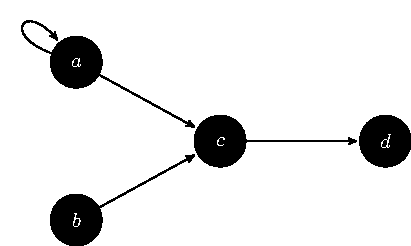
\includegraphics[scale=1.5]{graphs/ex4.pdf}
		\caption{An argumentation framework $F$, where $st(F)\subset sst(F)$}
	\end{figure}
\FloatBarrier

It can be computed that $adm(F)=\{\emptyset,\{b\},\{b,d\}\}$ and $co(F)=\{\{b,d\}\}$.\hl
There is no extension within $adm(F)$, that attacks all arguments it doesn't contain. Therefore $st(F)=\emptyset$.\hl
$\{b,d\}$ is the only complete extension, $\{b,d\}\cup \{c\}$ is maximal w.r.t. set inclusion, so it is semi-stable. It follows that $sst(F)=\{\{b,d\}\}$.\hl
As we can see (\ref{eq10}) is satisfied.\cl

\textbf{Example 11.} Let $F$ be an argumentation framework $(A,R)$ such that $A=\{a,b,c,d,e\}$ and $R=\{(a,b),(b,a),(b,c),(c,d),(d,e),(e,c)\}$\hl

\FloatBarrier
	\begin{figure}[!h]
		\centering
		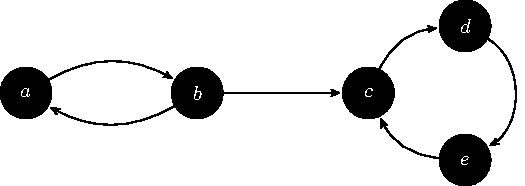
\includegraphics[width=\linewidth]{graphs/ex5.pdf}
		\caption{An argumentation framework $F$, where $sst(F)\subset prf(F)$}
	\end{figure}
\FloatBarrier

It can be computed that $co(F)=\{\emptyset,\{a\},\{b,d\}\}$ and $prf(F)=\{\{a\},\{b,d\}\}$.\hl
To obtain $sst(F)$ we need to compute $S\cup\{a\in A\text{ | } S\text{ attacks }a\}$ for all $S\in co(F)$. $\emptyset\cup\emptyset=\emptyset$, $\{a\}\cup\{b\}=\{a,b\}$ and $\{b,d\}\cup\{a,c,e\}=A$, only $A$ being maximal w.r.t. set inclusion. Therefore $sst(F)=\{\{b,d\}\}$.\hl
As we can see (\ref{eq11}) is satisfied.\cl

\subsection{Ideal extension}
There also is an alternative semantics to the grounded extension. Ideal extension semantics were introduced in \cite{Alferes} and also produce a unique sceptical set, albeit a less strict one.\hl

\textbf{Definition 11.} Let $S$ be an admissible extension. It is called the \emph{ideal extension} if it is the maximal (w.r.t. set inclusion) admissible extension contained in every preferred extension.\\
The ideal extension of an argumentation framework $F$ is denoted $id(F)$.\hl

Ideal extension is a superset of the grounded extension according to \cite{Dung2}. In \cite{Baroni} it is shown that the ideal extension is always a complete extension.

\begin{align}
	\label{eq12} gr(F)\subset id(F)\\
	\label{eq13} id(F)\in co(F)
\end{align}\hl

\textbf{Example 12.} Let $F$ be an argumentation $(A,R)$ such that $A=\{a,b,c,d,e\}$ and $R=\{(a,b),(b,d),(c,b),(d,a),(d,e),(e,c)\}$.\hl

\FloatBarrier
	\begin{figure}[!h]
		\centering
		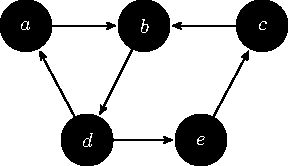
\includegraphics[scale=1.5]{graphs/ex6.pdf}
		\caption{An argumentation framework $F$, where $gr(F)\subset id(F)$ and $id(F)\in co(F)$}
	\end{figure}
\FloatBarrier

We know that $prf(F)=\{\{c,d\}\}$ and $co(F)=\{\emptyset,\{c,d\}\}$.\hl
It follows that $gr(F)=\emptyset$, while $id(F)=\{c,d\}$, so that (\ref{eq12}) and (\ref{eq13}) hold.\cl

\chapter{Implementation}

\section{Introduction}
In this chapter the usage and implementation details of the aforementioned program illustrating the computation of the different extension types is provided. The source code of the program as well as an executable .jar file can be found at \url{https://github.com/e1027108/bakk/}.  The program contains the following functionality:\hl

\begin{itemize}
\item Definition of argumentation frameworks
\item Loading of preset argumentation frameworks
\item Visualisation of argumentation frameworks as graphs
\item Computation of extensions (including step-by-step explanations)
\item Highlighting of extensions in the graph
\end{itemize}

The application consists of two views: the input mask and the graph view.

\section{Input mask}
On starting the application, the user is presented with an input mask. Here the user can choose from up to ten arguments. The number of arguments is limited because more than ten arguments don't provide any further benefit to a user wanting to learn about the basics of argumentation frameworks.\hl
There is a checkbox for every possible argument that is labelled with the name of the argument in capital letters ($A$ ... $J$). If a checkbox is selected the program will use the represented argument for further computations and visualisations.\hl
The user also has the option to give descriptions for arguments. They can be a strings of any form.\hl
Each argument has a textfield that contains the names of the arguments the argument in question attacks. Argument names are case-insensitive and can optionally be seperated either by ',' or spaces. Duplicate attacks are ignored. This means the attack fields accept the following syntax: \[[a-jA-J\text{ },]*\]\hl

There are some preset examples to be chosen from via the drop-down menu labelled ``choose preset''. Once an example is chosen, selection and text fields are updated corresponding to the chosen preset. Presets include examples given in \cite{Dung} and \cite{Egly} as well as examples used in this thesis.\hl
On clicking the ``show graph'' button, the application checks if the attack fields conform to the syntax for selected arguments and if they contain arguments that are not selected (meaning they don't exist and can therefore not be attacked). If there is invalid input an error message is displayed, if not the argumentation framework is created and the graph view displayed.\hl

\FloatBarrier
	\begin{figure}[!ht]
		\centering
		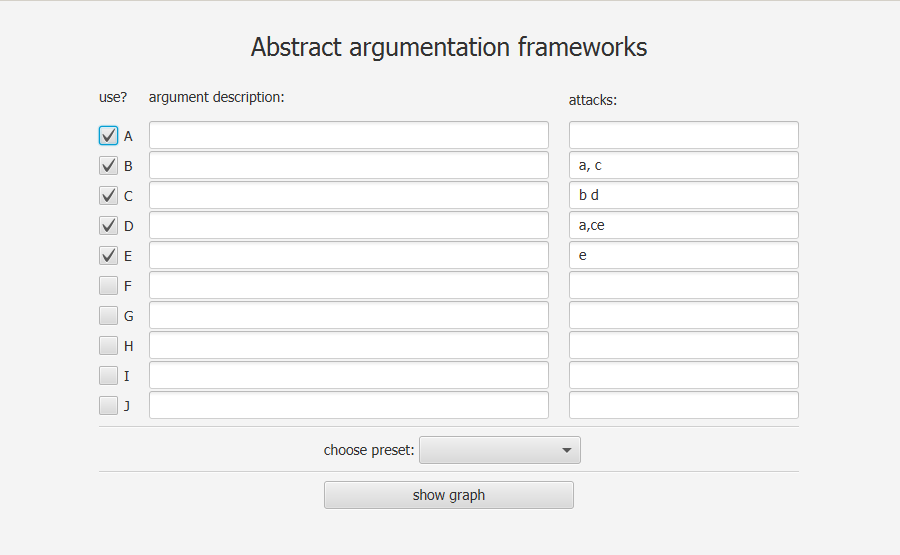
\includegraphics[width=\linewidth]{pics/chaotic.png}
		\caption{Input mask}
	\end{figure}
\FloatBarrier

Figure 4.1 shows the input mask with input representing the argumentation framework $F=(A,R)$ with $A=\{a,b,c,d\}$ and $R=\{(a,b),(b,c),(c,a),(d,b)\}$.\hl

\section{Graph view}

\FloatBarrier
	\begin{figure}[!h]
		\centering
		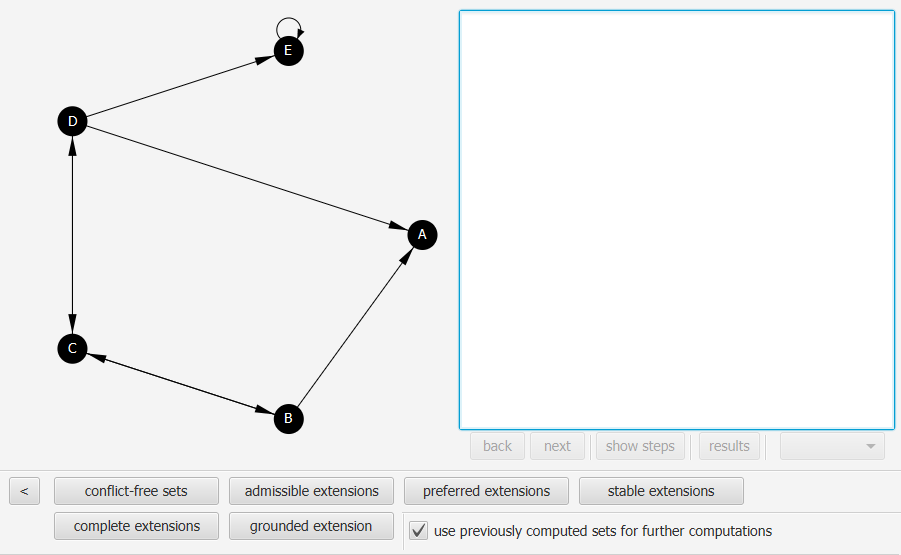
\includegraphics[width=\linewidth]{pics/graph.png}
		\caption{Graph view resulting from Figure 4.1}
	\end{figure}
\FloatBarrier

Upon loading the graph view (shown in Figure 4.2) the user can see the graph representing the argumentation framework defined in the input mask to the left. Every argument is represented by a node labelled with that arguments name. The argument nodes are arranged in a circle for better distinguishability.\hl
It is possible to view the arguments' descriptions by hovering over them. In case no description was given for an argument, the application displays this information.\hl

\FloatBarrier
	\begin{figure}[!h]
		\centering
		
\includegraphics[scale=2]{pics/argdes.png}
		\caption{Tooltip as shown hovering over an argument without description.}
	\end{figure}
\FloatBarrier

The user then has the option to choose to compute one of six types of sets:

\begin{itemize}[noitemsep]
	\item conflict-free set
	\item admissible extension
	\item preferred extension
	\item stable extension
	\item complete extension
	\item grounded extension
\end{itemize}

If the checkbox to ``use previously computed sets for further computations'' is selected, each computation takes into account the results of preceding computations, if applicable. If this option is not selected the program will compute every extension type needed, prior to computing the chosen extension.\\
That means if conflict-free sets were already computed one can compute stable extensions without the need to compute conflict-free sets again, but when trying to compute preferred extensions the set of admissible extensions would have to be freshly computed (the computation of the admissible extensions using the already computed conflict-free extensions).\hl
Each computation triggers the text area to the right (from now on called the explanation area) to display explanations of how the computed extensions came to pass. These explanations can either be shown step-by-step, all at once or be skipped so only the results of the computation are shown. Using previously computed extensions the explanation area does not show the explanation for already computed extensions again.\hl
Figure 4.4 shows the explanation shown during the computation of the complete extensions of the argumentation framework shown in Figure 4.1. Note that in this case, admissible extensions (as a prerequisite to compute complete extensions) did not need to be computed, because they had been computed beforehand.

\FloatBarrier
	\begin{figure}[!h]
		\centering
		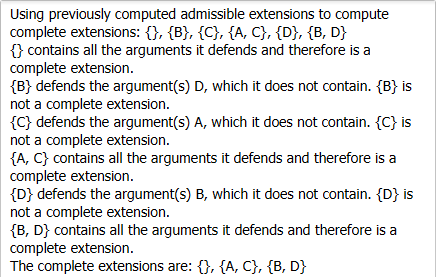
\includegraphics[scale=0.9]{pics/steps.png}
		\caption{Text explaining the computation of complete extensions.}
	\end{figure}
\FloatBarrier

To further illustrate the explanations shown the application recolours the graph for each step, using three easily distinguishable colours:\hl
Green is used for arguments included in the considered set and their relevant attacks needed to qualify for an extension type.\\
Red is used for conflicting arguments and attacks preventing a set of arguments from qualifying for an extension type.\\
Blue is used for arguments missing from a set for it to qualify for an extension type.\hl
Figure 4.5 is an example where all three colours are used to illustrate the applications reasoning in computing complete extensions.\hl

\FloatBarrier
	\begin{figure}[!h]
		\centering
		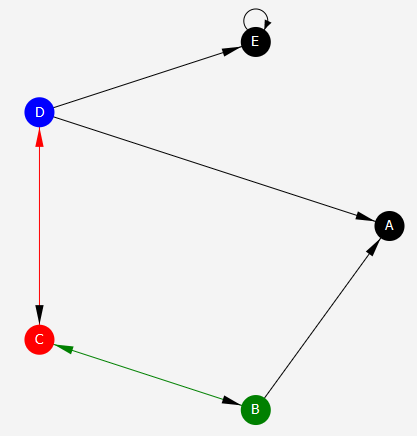
\includegraphics{pics/missing.png}
		\caption[Highlighting of nodes and edges in a graph]{$\{B\}$ defends the argument $D$, which it does not contain. $\{B\}$ is not a complete extension.}
	\end{figure}
\FloatBarrier

After showing the results of a computation a dropdown menu becomes availiable beneath the right bottom corner of the explanation area, containing all computed extensions. They can be selected and are then highlighted in green in the graph.\hl
The graph view also allows the user to go back to the input mask using the `<' button. The input mask still contains the input from before switching to the graph view to allow the user to make small adjustments without having to redefine the whole framework.

\section{Implementation details}
This section lists which technologies where used to create the program, what class structure was used to represent argumentation frameworks and what these classes do.\cl

\subsection{Technologies and Resources used}
The application was written in Java (version 1.8) using eclipse Kepler as a working environment.\hl
As the graphical user interface JavaFX was used, the design being created as .fxml files via JavaFX Scene Builder.\hl
Java Universal Network/Graph Framework (JUNG) was used for the data structure of the graphs.

\subsection{Program structure}
There exist four classes in the application which model argumentation frameworks:

\begin{itemize}[noitemsep]
	\item Argument.java
	\item Attack.java
	\item Framework.java
	\item Extension.java
\end{itemize}

These classes have the following relationships:

\FloatBarrier
\begin{figure}[!h]
	\centering
	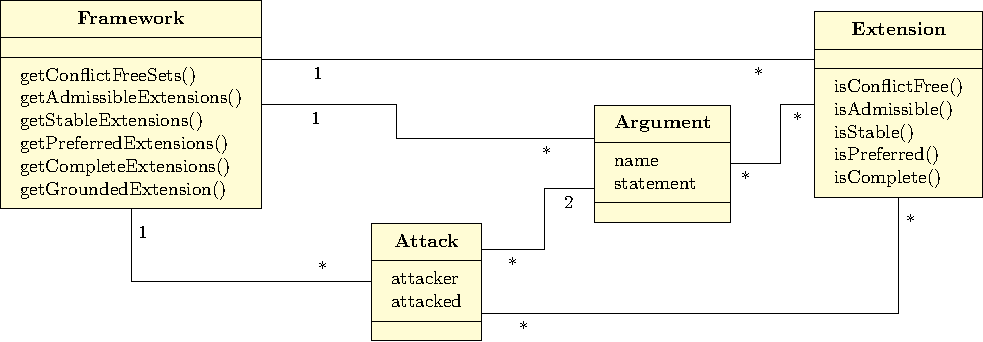
\includegraphics[width=\linewidth]{graphs/classes.pdf}
	\caption{Argumentation framework class diagram}
\end{figure}
\FloatBarrier

\subsubsection{Argument}
An \emph{Argument} object is a pair consisting of a key and a value. The key is the name of the argument (representing an argument $a\in A$), while the value is the argument's statement.

\subsubsection{Attack}
An \emph{Attack} object stores a pair of Argument objects. The first argument is called the ``attacker'', the second the ``attacked'' argument representing an attack $(a,b)\in R$.

\subsubsection{Framework}
A \emph{Framework} object represents an argumentation framework $F=(A,R)$. It contains a list of all arguments ($A$) and a list of all attacks ($R$). It also stores all the extensions.\hl
If a user wants to compute the extensions of a specific type (except the grounded extension), the framework calls the corresponding method of every extension candidate to find out if it indeed is of that extension type. For this purpose the framework can store multiple lists of extension candidates (e.g. The framework can store a list of conflict-free sets, which then can be used to compute admissible or stable extensions). After each candidate has returned its status, the frameworks returns a list of extensions that satisfy the criteria of the extension type in question.\hl
To compute the grounded extension the framework simply compares the arguments of its complete extensions, without any algorithms of the extension object being called.

\subsubsection{Extension}
An \emph{Extension} object represents a set $S\subseteq A$. For that purpose it stores a list of Argument objects. Every extension object stores a reference to the framework it belongs to, to compute and store lists of outgoing and incoming attacks.\hl
Each extension object can compute if it is of a certain extension type (except for grounded extensions, see above).

\backmatter

\listoffigures

%\bibliographystyle{alpha}
%\bibliography{intro}
\printbibliography

%\printindex
%\printglossaries

\end{document}